\documentclass[aspectratio=169,11pt]{beamer}

\usetheme{Madrid}
\usecolortheme{default}

\usepackage[T1]{fontenc}
\usepackage[utf8]{inputenc}
\usepackage{amsmath,amssymb,bm}
\usepackage{booktabs}
\usepackage{tikz}
\usetikzlibrary{arrows.meta,positioning,fit}

% Change to show notes if you want speaker notes in the generated PDF.
% Options:
%   \setbeameroption{hide notes}
%   \setbeameroption{show notes}
\setbeameroption{hide notes}

\title[Robust KalmaNet for QCar]{Robust KalmaNet State Estimation for QCar}
\subtitle{Physics Prediction + Learned Robust GPS/Velocity Update}
\author{Quang Huy Nugyen}
\institute{Multi-Vehicle Self-Driving Real QCar Project}
\date{\today}

\newcommand{\state}{\bm{x}}
\newcommand{\meas}{\bm{z}}
\newcommand{\pred}{\state_k^-}
\newcommand{\upd}{\state_k^+}
\newcommand{\wrap}{\operatorname{wrap}}
\newcommand{\diag}{\operatorname{diag}}

\begin{document}

% ------------------------------------------------------------
\begin{frame}
  \titlepage

  \vspace{-0.5em}
  \begin{center}
    \small
    RKNet estimates $\state=[x,y,\psi,v]^T$ while rejecting corrupted GPS and velocity measurements.
  \end{center}

  \note{
    This presentation explains the Robust KalmaNet implementation in the
    Robust folder. The key message is that the estimator is not a fully
    black-box network. It uses a QCar kinematic prediction model and a learned
    Kalman-style update that can reduce trust in corrupted GPS or velocity.
  }
\end{frame}

% ------------------------------------------------------------
\begin{frame}{Problem Setup: Signals and Measurement}
  \begin{block}{Measurement vector}
    \[
      \meas_k =
      \begin{bmatrix}
        x_{gps,k} & y_{gps,k} & \psi_{fused,k} & v_{tach,k}
      \end{bmatrix}^{T}
    \]
  \end{block}

  \begin{columns}[T,onlytextwidth]
    \column{0.49\textwidth}
    \textbf{Raw branch inputs}
    \begin{itemize}
      \item IMU: $[v,\psi,a_x,a_y,\omega_z]$
      \item Steering: $[v,\psi,\delta]$
      \item Wheel: $[v,\psi,v_{fl},v_{fr},v_{rl},v_{rr}]$
    \end{itemize}

    \column{0.49\textwidth}
    \textbf{Availability information}
    \begin{itemize}
      \item GPS position valid flag
      \item Heading valid flag
      \item GPS hold valid flag
      \item GPS age in seconds
    \end{itemize}
  \end{columns}

  \vspace{0.5em}
  \begin{block}{Observation model}
    \[
      \meas_k = H\state_k + \bm{n}_k,
      \qquad
      H \approx I_4
    \]
  \end{block}

  \note{
    The implementation uses state order x, y, heading, velocity. The
    measurement has the same four channels. The heading measurement is rebuilt
    using the local QCar heading fusion path, and GPS validity metadata is kept
    because it is essential for robust update behavior.
  }
\end{frame}

% ------------------------------------------------------------
\begin{frame}{RKNet Concept Design}
  \begin{center}
    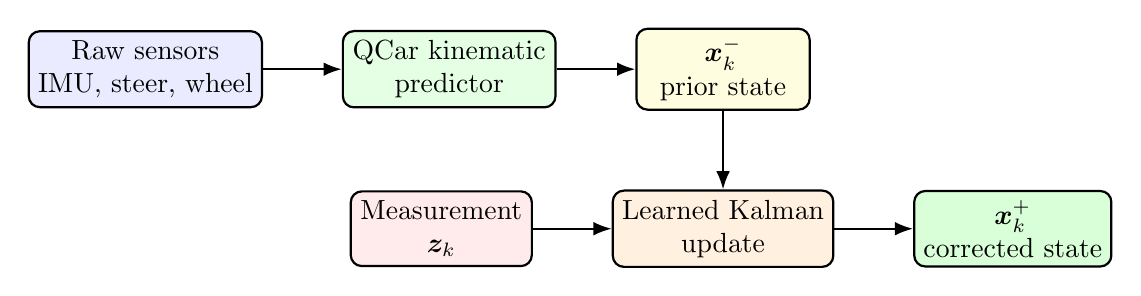
\begin{tikzpicture}[node distance=0.9cm and 1.0cm,>=Latex,thick]
      \node[draw,rounded corners,align=center,fill=blue!8,minimum width=2.4cm,minimum height=0.8cm] (raw) {Raw sensors\\IMU, steer, wheel};
      \node[draw,rounded corners,right=of raw,align=center,fill=green!10,minimum width=2.7cm,minimum height=0.8cm] (pred) {QCar kinematic\\predictor};
      \node[draw,rounded corners,right=of pred,align=center,fill=yellow!12,minimum width=2.2cm,minimum height=0.8cm] (xp) {$\state_k^-$\\prior state};

      \node[draw,rounded corners,below=1.0cm of xp,align=center,fill=orange!12,minimum width=2.8cm,minimum height=0.8cm] (upd) {Learned Kalman\\update};
      \node[draw,rounded corners,left=of upd,align=center,fill=red!8,minimum width=2.3cm,minimum height=0.8cm] (z) {Measurement\\$\meas_k$};
      \node[draw,rounded corners,right=of upd,align=center,fill=green!15,minimum width=2.2cm,minimum height=0.8cm] (xu) {$\state_k^+$\\corrected state};

      \draw[->] (raw) -- (pred);
      \draw[->] (pred) -- (xp);
      \draw[->] (xp) -- (upd);
      \draw[->] (z) -- (upd);
      \draw[->] (upd) -- (xu);
    \end{tikzpicture}
  \end{center}

  \begin{itemize}
    \item Current configuration uses \texttt{predictor\_mode: kinematic}.
    \item Prediction is physics-based, not learned.
    \item Update learns measurement reliability mask and Kalman gain.
    \item Main robustness target: GPS position and velocity corruption.
  \end{itemize}

  \note{
    The code supports a neural predictor, but the active training config uses
    the kinematic predictor. That is important for the story: the vehicle
    motion prior comes from the QCar model, and learning focuses on robust
    correction.
  }
\end{frame}

% ------------------------------------------------------------
\begin{frame}{Prediction Math: QCar Bicycle Model}
  \small
  \begin{block}{Yaw-rate and local motion}
    \[
      \dot{\psi}_k =
      \frac{v_{pose,k}\tan(\delta_k)}{L},
      \qquad
      \Delta x_E = v_{pose,k}\Delta t,
      \qquad
      \Delta y_E = 0
    \]
  \end{block}

  \begin{block}{Global prediction}
    \vspace{-0.4em}
    \[
      x_k^- = x_{k-1}^+ + v_{pose,k}\cos(\psi_{k-1}^+)\Delta t
    \]
    \[
      y_k^- = y_{k-1}^+ + v_{pose,k}\sin(\psi_{k-1}^+)\Delta t
    \]
    \[
      \psi_k^- =
      \wrap\left(\psi_{k-1}^+
      + \frac{v_{pose,k}\tan(\delta_k)}{L}\Delta t\right)
    \]
    \vspace{-0.8em}
  \end{block}

  \begin{block}{Velocity lag model used by current config}
    \vspace{-0.6em}
    \[
      a_k =
      \frac{-v_{k-1}^{+} + g u_k}{\tau},
      \qquad
      v_k^- =
      \operatorname{clip}
      \left(v_{k-1}^{+}+a_k\Delta t\right)
    \]
    \vspace{-0.8em}
  \end{block}

  \vspace{-0.5em}
  \small
  Config values: $L=0.2$, $\tau=0.301$, $g=6.598$, $|v|\leq 2.0$.

  \note{
    This slide explains what the prediction step contributes. The predictor
    estimates where the car should move according to velocity, steering, and
    throttle. This gives a reasonable prior before the GPS and velocity
    measurements are used.
  }
\end{frame}

% ------------------------------------------------------------
\begin{frame}{Learned Robust Update Math}
  \scriptsize
  \begin{columns}[T,onlytextwidth]
    \column{0.52\textwidth}
    \begin{block}{Innovation}
      \[
        \bm{r}_k = \wrap(\meas_k - H\state_k^-),
        \qquad
        \Delta\meas_k = \wrap(\meas_k-\meas_{k-1})
      \]
    \end{block}

    \begin{block}{Updater features}
      \[
      \begin{aligned}
        \Delta\state_k &= \wrap(\state_k^- - \state_{k-1}^{+}) \\
        \bar{\bm{r}}_k &= \bm{a}_k \odot \bm{r}_k,\qquad
        \bar{\Delta\meas}_k = \bm{a}_k \odot \Delta\meas_k \\
        \eta_k &= \log(1+\min(age_k,10))
      \end{aligned}
      \]
      \[
        \bm{f}_k =
        \left[
        \frac{\Delta\state_k}{\bm{s}_x},
        \frac{\bar{\bm{r}}_k}{\bm{s}_z},
        \frac{\bar{\Delta\meas}_k}{\bm{s}_z},
        \bm{a}_k,
        g_k^{hold},
        \eta_k,
        \log(1+|\bar{\bm{r}}_k|),
        \log(1+|\bar{\Delta\meas}_k|)
        \right]
      \]
      For $[x,y,\psi,v]$, $\bm{a}_k=[g_k,g_k,h_k,1]^T$ and
      $\bm{f}_k\in\mathbb{R}^{26}$.
    \end{block}

    \column{0.46\textwidth}
    \begin{block}{Measurement mask}
      \[
        \bm{m}_k^z =
        \sigma(MLP(\bm{f}_k))
      \]
      \[
        \tilde{\bm{r}}_k =
        \bm{m}_k^z \odot \bm{a}_k \odot \bm{r}_k
      \]
    \end{block}

    \begin{block}{Learned Kalman gain}
      \[
        \bm{h}_k =
        GRU(\bm{m}_k \odot \bm{f}_k,\bm{h}_{k-1})
      \]
      \[
        K_k =
        s\tanh(MLP(\bm{h}_k))
      \]
    \end{block}
  \end{columns}

  \begin{block}{Final update}
    \[
      \state_k^+ = \state_k^- + K_k\tilde{\bm{r}}_k
    \]
  \end{block}

  \note{
    The most important part is the masked innovation. Even if GPS gives a
    large position jump or velocity is corrupted, the update can reduce that
    channel before applying the learned gain. This makes the correction more
    conservative and more interpretable.
  }
\end{frame}

% ------------------------------------------------------------
\begin{frame}{Attack Setup: Focus on GPS and Velocity}
  \small
  \begin{columns}[T,onlytextwidth]
    \column{0.48\textwidth}
    \textbf{GPS position attacks}
    \begin{itemize}
      \item Noise: $z_{xy}^{atk}=z_{xy}+\epsilon$
      \item Jump: $z_{xy}^{atk}=z_{xy}+\bm{b}_{jump}$
      \item Freeze: $z_{xy,k}^{atk}=z_{xy,k_0}$
      \item Dropout: $gps\_valid_k=0$
      \item Reacquisition offset
    \end{itemize}

    \column{0.48\textwidth}
    \textbf{Velocity attacks}
    \begin{itemize}
      \item Bias: $z_v^{atk}=z_v+b_v$
      \item Scale: $z_v^{atk}=\alpha z_v$
      \item Freeze: $z_{v,k}^{atk}=z_{v,k_0}$
      \item Noise, ramp, or zero-out
      \item Wheel branch: $v_{fl},v_{fr},v_{rl},v_{rr}$
    \end{itemize}
  \end{columns}

  \vspace{0.3em}
  \begin{block}{Current augmentation probabilities}
    \vspace{-0.5em}
    \[
      \begin{aligned}
      P(GPS)&=0.45, &
      P(direct\ meas.)&=0.35, &
      P(raw\ branch)&=0.25
      \end{aligned}
    \]
    \vspace{-0.8em}

    Maximum attacked raw branches per sample: $1$.
  \end{block}

  Expected behavior:
  $\bm{m}_{k,i}^{z}\approx 1$ for clean channels and
  $\bm{m}_{k,i}^{z}\approx 0$ for attacked GPS/velocity channels.

  \note{
    This is the attack slide to emphasize in the talk. The training does not
    treat every sensor fault equally. GPS position and velocity are the main
    robustness targets because they directly affect the state correction.
    GPS attacks teach the model not to snap to a bad position. Velocity attacks
    teach the model not to over-correct speed when wheel or tachometer
    measurements become unreliable.
  }
\end{frame}

% ------------------------------------------------------------
\begin{frame}{Dataset and Training}
  \scriptsize
  \begin{columns}[T,onlytextwidth]
    \column{0.48\textwidth}
    \textbf{Dataset generation}
    \begin{itemize}
      \item Recorder saves \texttt{datasets/*.npz} and \texttt{*.json}.
      \item Saved fields: raw sensors, GPS flags, $\meas_k$, target $\state_k^\ast$, timestamps.
      \item Active example: \texttt{V0\_20260417\_094048.npz}
    \end{itemize}

    \[
      \{raw,\meas,\state^\ast,\state_0,\Delta t\}
      \rightarrow
      [t:t+T]
    \]

    \column{0.50\textwidth}
    \textbf{Training schedule}
    \begin{itemize}
      \item $T=50$, Phase C $T=80$, stride $1$.
      \item Validation split: $20\%$ tail.
      \item Phase A: predictor only, skipped for kinematic predictor.
      \item Phase B: train updater only.
      \item Phase C: runtime-style fine tuning, teacher forcing off.
    \end{itemize}
  \end{columns}

  \begin{block}{Loss: accuracy + robust correction behavior}
    \vspace{-0.9em}
    \[
    \begin{aligned}
      \mathcal{L} &=
      \lambda_u L_{upd}
      + \lambda_p L_{pred}
      + \lambda_m L_{mask}
      + \lambda_K L_{gain}
      + \lambda_{\Delta K}L_{\Delta K}
      + \lambda_{\Delta m}L_{\Delta m}
    \end{aligned}
    \]
    \[
    \begin{aligned}
      L_{upd} &= MSE_W(\state^+,\state^\ast),
      &L_{pred} &= MSE_W(\state^-,\state^\ast) \\
      L_{mask} &= BCE(\bm{m}^z,1-\bm{\ell}^{atk}),
      &L_{gain} &= \|K\|_2^2 \\
      L_{\Delta K} &= \|K_k-K_{k-1}\|_2^2,
      &L_{\Delta m} &= \|\bm{m}_k^z-\bm{m}_{k-1}^z\|_2^2
    \end{aligned}
    \]
    \vspace{-0.9em}
  \end{block}

  \begin{columns}[T,onlytextwidth]
    \column{0.52\textwidth}
    \textbf{Meaning}
    \begin{itemize}
      \item $L_{upd}$: final corrected state should match the reference.
      \item $L_{pred}$: prior prediction should stay physically reasonable.
      \item $L_{mask}$: clean channel target $=1$, attacked channel target $=0$.
    \end{itemize}

    \column{0.46\textwidth}
    \textbf{Stability terms}
    \begin{itemize}
      \item $L_{gain}$: avoid very large Kalman gains.
      \item $L_{\Delta K}$: avoid gain chatter.
      \item $L_{\Delta m}$: avoid mask flicker.
    \end{itemize}
  \end{columns}

  Current weights: $\lambda_u=0.85$, $\lambda_p=0.15$,
  $W=[1.0,1.0,2.5,1.2]$, $\lambda_K=0.01$,
  $\lambda_{\Delta K}=0.02$.

  \note{
    The dataset recorder stores clean real driving data. During offline
    training, synthetic GPS and velocity attacks are injected to create
    supervised examples of corrupted channels. The loss both minimizes state
    error and teaches the measurement mask to reject attacked channels.
  }
\end{frame}

% ------------------------------------------------------------
\begin{frame}{Testing, Diagnostics, and Result}
  \small
  \begin{block}{Evaluation metric}
    \vspace{-0.6em}
    \[
      RMSE_i =
      \sqrt{
        \frac{1}{N}
        \sum_{k=1}^{N}
        \left(
          \hat{x}_{k,i}-x_{k,i}^{\ast}
        \right)^2
      }
    \]
    \vspace{-0.8em}
  \end{block}

  \begin{columns}[T,onlytextwidth]
    \column{0.47\textwidth}
    \textbf{Compared methods}
    \begin{itemize}
      \item QCar kinematic reference
      \item Learned RKNet checkpoint
      \item Target EKF/reference state
    \end{itemize}

    \column{0.50\textwidth}
    \textbf{Saved validation after timestamp fix}
    \begin{table}
      \centering
      \small
      \begin{tabular}{lc}
        \toprule
        Method & Mean RMSE \\
        \midrule
        Kinematic reference & 0.152 \\
        Learned RKNet & 0.070 \\
        \bottomrule
      \end{tabular}
    \end{table}
  \end{columns}

  \vspace{0.1em}
  \textbf{Diagnostics:} state error, GPS/velocity mask, masked innovation, and Kalman gain during attack/recovery.

  \vspace{0.2em}
  \textbf{Takeaway:} RKNet keeps QCar physics, but learns when to trust GPS and velocity.

  \note{
    Offline validation command:
    python validate_robust_kalmannet.py
    datasets\textbackslash robust_kalmannet_dataset_V0_20260417_094048.npz
    --checkpoint models\textbackslash robust_kalmannet.best_robust.pt
    --sequence-length 50 --device auto.

    For the final presentation, show one plot where GPS or velocity is attacked.
    The important visual evidence is that the measurement mask drops during
    attack, the masked innovation becomes smaller than the raw innovation, and
    the state estimate recovers without a large jump. The saved validation file
    already reports lower mean RMSE for RKNet than the kinematic reference.
  }
\end{frame}

\end{document}
